 \let\negmedspace\undefined
\let\negthickspace\undefined
\documentclass[journal]{IEEEtran}
\usepackage[a5paper, margin=10mm, onecolumn]{geometry}
%\usepackage{lmodern} % Ensure lmodern is loaded for pdflatex
\usepackage{tfrupee} % Include tfrupee package

\setlength{\headheight}{1cm} % Set the height of the header box
\setlength{\headsep}{0mm}     % Set the distance between the header box and the top of the text

\usepackage{gvv-book}
\usepackage{gvv}
\usepackage{cite}
\usepackage{amsmath,amssymb,amsfonts,amsthm}
\usepackage{algorithmic}
\usepackage{graphicx}
\usepackage{textcomp}
\usepackage{xcolor}
\usepackage{txfonts}
\usepackage{listings}
\usepackage{enumitem}
\usepackage{mathtools}
\usepackage{gensymb}
\usepackage{comment}
\usepackage[breaklinks=true]{hyperref}
\usepackage{tkz-euclide} 
\usepackage{listings}
% \usepackage{gvv}                                        
\def\inputGnumericTable{}                                 
\usepackage[latin1]{inputenc}                                
\usepackage{color}                                            
\usepackage{array}                                            
\usepackage{longtable}                                       
\usepackage{calc}                                             
\usepackage{multirow}                                         
\usepackage{hhline}                                           
\usepackage{ifthen}                                           
\usepackage{lscape}
\usepackage{circuitikz}
\tikzstyle{block} = [rectangle, draw, fill=blue!20, 
    text width=4em, text centered, rounded corners, minimum height=3em]
\tikzstyle{sum} = [draw, fill=blue!10, circle, minimum size=1cm, node distance=1.5cm]
\tikzstyle{input} = [coordinate]
\tikzstyle{output} = [coordinate]
\renewcommand{\thefigure}{\theenumi}
\renewcommand{\thetable}{\theenumi}
\setlength{\intextsep}{10pt} % Space between text and floats
\numberwithin{equation}{enumi}
\numberwithin{figure}{enumi}
\renewcommand{\thetable}{\theenumi}

\begin{document}

\bibliographystyle{IEEEtran}
\vspace{3cm}

\title{1.5.16}
\author{EE25BTECH11028 - J.Navya sri}
\maketitle

\subsection*{\textbf{Question:} } 
Find the coordinates of a point $A$ where $AB$ is the diameter of the circle with center is $\myvec{3\\-1 }$ and $B$ is the point $\myvec{2\\6}.$\\
\solution \\ 
Given data:
\[
\begin{tabular}[12pt]{ |c| c| c|} 
    \hline
    {Point} & {Vector} \\ 
    \hline
    B & $ \myvec{2 \\ 6} $  \\
    \hline
     P & $ \myvec{3 \\ -1} $   \\
    \hline  
    \end{tabular}
\]

\underline{\textbf{Theory :}} Center of a circle is the mid-point of the diameter. \\

Let $P$ be the center of the given circle , with $AB$ as the diameter.

Let $\vec{A}$ be the Vector to be found 

\textit{Given :} 
\[
B \equiv \begin{pmatrix} 2 \\ 6 \end{pmatrix}, \quad P \equiv \begin{pmatrix} 3 \\ -1 \end{pmatrix}
\]
Center of a circle is the mid point of the diameter. For a circle with center $\vec{P}$ and ends of diameters represented by vectors $\vec{A}$ and $\vec{B}$  
\[
\mathbf{P} = \frac{\mathbf{A} + \mathbf{B}}{2} \tag{0.1}
\]

Rearranging , we get:
\[
\mathbf{A} = 2\mathbf{P} - \mathbf{B} \tag{0.2}
\]

Substituting the given vectors, we get:
\[
\mathbf{A} = 2 \begin{pmatrix} 3 \\ -1 \end{pmatrix} - \begin{pmatrix} 2 \\ 6 \end{pmatrix} \tag{0.3}
\]
\[
\mathbf{A} = \begin{pmatrix} 6 \\ -2 \end{pmatrix} - \begin{pmatrix} 2 \\ 6 \end{pmatrix} \tag{0.4}
\]
\[
\therefore \mathbf{A} \equiv \begin{pmatrix} 4 \\ -8 \end{pmatrix}
\]

\textbf{Hence , Coordinates of A are } 
\[
\begin{pmatrix} 4 \\ -8 \end{pmatrix}
\]


\textbf{Graph representation:}
\begin{figure}[H]
    \centering
 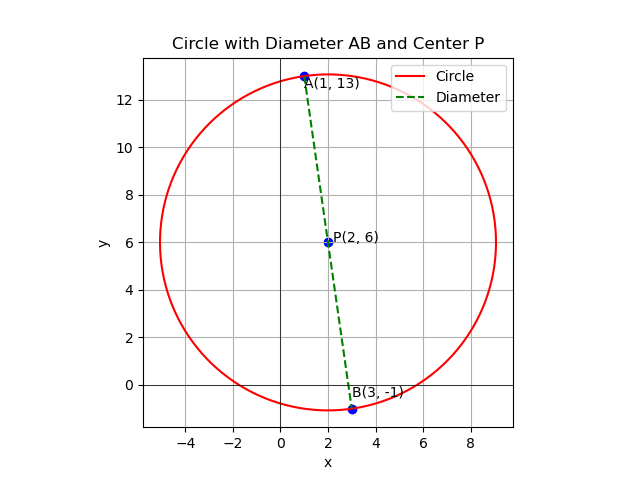
\includegraphics[width=0.5\linewidth]{figs/fig1.png}
    \caption{}
    \label{fig:placeholder}
\end{figure}
\end{document}


